%% This is file `elsarticle-template-1-num.tex',
%%
%% Copyright 2009 Elsevier Ltd
%%
%% This file is part of the 'Elsarticle Bundle'.
%% ---------------------------------------------
%%
%% It may be distributed under the conditions of the LaTeX Project Public
%% License, either version 1.2 of this license or (at your option) any
%% later version.  The latest version of this license is in
%%    http://www.latex-project.org/lppl.txt
%% and version 1.2 or later is part of all distributions of LaTeX
%% version 1999/12/01 or later.
%%
%% Template article for Elsevier's document class `elsarticle'
%% with numbered style bibliographic references
%%
%% $Id: elsarticle-template-1-num.tex 149 2009-10-08 05:01:15Z rishi $
%% $URL: http://lenova.river-valley.com/svn/elsbst/trunk/elsarticle-template-1-num.tex $
%%

%% Use the option review to obtain double line spacing
%% \documentclass[preprint,review,12pt]{elsarticle}

%% Use the options 1p,twocolumn; 3p; 3p,twocolumn; 5p; or 5p,twocolumn
%% for a journal layout:
%% \documentclass[final,1p,times]{elsarticle}
%% \documentclass[final,1p,times,twocolumn]{elsarticle}
%% \documentclass[final,3p,times]{elsarticle}
%% \documentclass[final,3p,times,twocolumn]{elsarticle}
%% \documentclass[final,5p,times]{elsarticle}
%% \documentclass[final,5p,times,twocolumn]{elsarticle}
%% The lineno packages adds line numbers. Start line numbering with
%% \begin{linenumbers}, end it with \end{linenumbers}. Or switch it on
%% for the whole article with \linenumbers after \end{frontmatter}.%% natbib.sty is loaded by default. However, natbib options can be
%% provided with \biboptions{...} command. Following options are
%% valid:


%%   round  -  round parentheses are used (default)
%%   square -  square brackets are used   [option]
%%   curly  -  curly braces are used      {option}
%%   angle  -  angle brackets are used    <option>
%%   semicolon  -  multiple citations separated by semi-colon
%%   colon  - same as semicolon, an earlier confusion
%%   comma  -  separated by comma
%%   numbers-  selects numerical citations
%%   super  -  numerical citations as superscripts
%%   sort   -  sorts multiple citations according to order in ref. list
%%   sort&compress   -  like sort, but also compresses numerical citations
%%   compress - compresses without sorting
%%
%% \biboptions{comma,round}

% \biboptions{}
%% use the tnoteref command within \title for footnotes;
%% use the tnotetext command for the associated footnote;
%% use the fnref command within \author or \address for footnotes;
%% use the fntext command for the associated footnote;
%% use the corref command within \author for corresponding author footnotes;
%% use the cortext command for the associated footnote;
%% use the ead command for the email address,
%% and the form \ead[url] for the home page:
%%
%% \title{Title\tnoteref{label1}}
%% \tnotetext[label1]{}
%% \author{Name\corref{cor1}\fnref{label2}}
%% \ead{email address}
%% \ead[url]{home page}
%% \fntext[label2]{}
%% \cortext[cor1]{}
%% \address{Address\fnref{label3}}
%% \fntext[label3]{}


%% use optional labels to link authors explicitly to addresses:
%% \author[label1,label2]{<author name>}
%% \address[label1]{<address>}
%% \address[label2]{<address>}

%% Authors are advised to submit their bibtex database files. They are
%% requested to list a bibtex style file in the manuscript if they do
%% not want to use model1-num-names.bst.

%% The amsthm package provides extended theorem environments
%% The graphicx package provides the includegraphics command.
%% The amssymb package provides various useful mathematical symbols

%% References without bibTeX database:

% \begin{thebibliography}{00}

%% \bibitem must have the following form:
%%   \bibitem{key}...
%%

% \bibitem{}

% \end{thebibliography}

%%
%% End of file `elsarticle-template-1-num.tex'.
\documentclass[preprint]{elsarticle}



\usepackage{graphicx}

\usepackage{amssymb}

%% \usepackage{amsthm}
\usepackage{caption}
\usepackage{floatrow}


\usepackage{lineno}
\usepackage[a4paper, total={6in, 8in}]{geometry}
\usepackage{wrapfig}
\usepackage{multicol}
\usepackage{xcolor}
\usepackage{subcaption}


\newfloatcommand{capbtabbox}{table}[][\FBwidth]
\newcommand{\todo}[1]{{\color{red}#1}}

\journal{ANZCOP}

\begin{document}

\begin{frontmatter}

\title{Precision measurement of weak transitions from excited states in Helium by counting ultracold atoms}

\author{J. A. Ross, K. F. Thomas, B. M. Henson, S. S. Hodgman, A. Truscott, K. G. H. Baldwin}
\address{ Laser Physics Centre, Research School of Physics and Engineering, The Australian National University, Canberra, ACT 2601, Australia
}%$^2 $Physics Department, University of Windsor, Windsor, Ontario, Canada}
\date{}
\begin{keyword}
Frequency metrology \sep Atomic spectroscopy \sep Bose-Einstein Condensate \sep Metastable Helium \sep Precision Measurement

\end{keyword}


\end{frontmatter}



The advancing precision of modern atomic spectroscopy is beginning to afford optical tests of fundamental physics in helium through, for instance, nuclear charge radii determinations\cite{Pachucki2017}. Helium therefore provides a testbed as appealing as Hydrogen for spectroscopic tests of QED. Among outstanding discrepancies between predicted and observed Helium transition lines are the 7.5$\sigma$ difference in the $n=3$ singlet-triplet splitting\cite{Luo2015} and the $93\sigma$ difference between Martin's measurements of the $2^3P_2 \rightarrow 5^3S_1$ and $2^3P_2 \rightarrow5^3D$ transitions values, and recent predictions by Drake \cite{Drake2007}.
We contribute to both of these by measuring five transitions from the $2^3P_2$ state, improving on Martin's measurements with an order of magnitude greater precision, and making the first observation of the spin-forbidden $2^3P_2\rightarrow5^1D_2$ transition in Helium. Our measurements constrain  the $5^3D$ and $5^1D$ ionization energies of 4He\cite{Morton2006} to 150 parts per billion, and the $5^3S$ to 28 parts per billion.

\begin{wrapfigure}{l}{0.5\textwidth}
    \begin{center}
        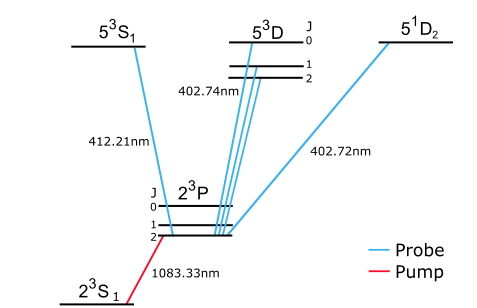
\includegraphics[width=\textwidth]{lvl_diag.png}    
    \end{center}
    \caption{Level diagram showing the measured transitions from the $2^3\mathrm{P}_2$ state to the $n=5$ manifold (blue), after pumping from the metastable $2^3\mathrm{S}_1$ state in an optical molasses.\\
    }
    \label{fig:my_label}
\end{wrapfigure}

We use a novel spectroscopic technique for direct, low-background laser spectroscopy of excited state transitions. We apply a probe beam during the optical cooling of ultracold trapped atoms to disturb the cooling process, with the cooling beam acting also as the optical pump. Evaporative cooling transforms this disturbance into change in a final atom number, which we measure with our single-atom sensitive detector. We identify the transition frequency as the peak of the change in atom number with respect to probe beam frequency. This method is advantageous for studying excited-state transitions as it provides an essentially background-free measurement protocol which is, in principle, sensitive to absorption of single photons. Further, the experiments are performed in a controlled magnetic field for precise calibration of Zeeman shifts, and in ultra-high vacuum with densities low enough such that the pressure shift is minimal. 

The predicted transition frequencies\cite{Pachucki2017} agree with the observed values within experimental error, which is ultimately limited by the absolute accuracy of our High Finesse WS-8 wave meter. The widths of the observed peaks agree well with the predicted natural linewidths.  We discuss potential extensions of this method to measure decay branching ratios, lifetimes, and oscillator strengths, sub-Doppler spectrometry, and the prospect of isotope-shift measurements in 3He-4He mixtures.

%% Aligned horizontally
%% https://tex.stackexchange.com/questions/120296/how-to-manipulate-width-and-position-of-items-inside-floatrow
\begin{figure}[h]
\begin{floatrow}
\ffigbox[][]
    {\caption{Observed $ 2^3P_2 \rightarrow5^1D_2$ transition peak in uniform magnetic fields of strength 18G (left) and 11G  (right). This singlet-triplet transition has a predicted oscillator strength five orders of magnitude weaker than that of the cooling (pump) transition, with accurate Lorentzian fits.}}
    {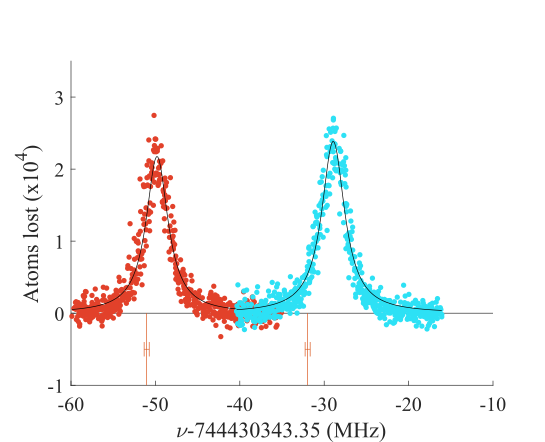
\includegraphics[width=0.5\textwidth]{5^1D_2_plot_combo.png}}
    \capbtabbox{%
  \begin{tabular}{|c||c|c|c|p{1cm}}
    \hline
        Upper state &  $\nu_{obs}$ (MHz)     & $ \nu_{obs} - \nu_{old}\cite{Martin60}$\\
    \hline\hline
        $5^3\mathrm{S}_1$    & 727303247(4)        & 13713(201)\\
        $5^3\mathrm{D}_1$    & 744396515(20)        & 13575(168)\\
        $5^3\mathrm{D}_2$    & 744396235(20)        & 13855(168)\\
        $5^3\mathrm{D}_3$    & 744396204(20)        & 13886(168)\\
        $5^1\mathrm{D}_2$    & 744430345(20)        & N/A\\
        \hline
    \end{tabular}
    \newline\newline\newline\newline
}{%
  \caption{Results of our measurements of transition frequencies between the $2^3\textrm{P}_2$ state to the listed upper states. Uncertainty in observed frequency is dominated by the limiting wavemeter accuracy. The uncertainty in the difference between new values and Martin's results \cite{Martin60} is the combined uncertainty of both measurements.}
}
\end{floatrow}
\end{figure}

%% Stacked vertically
% \begin{figure}[h]
% 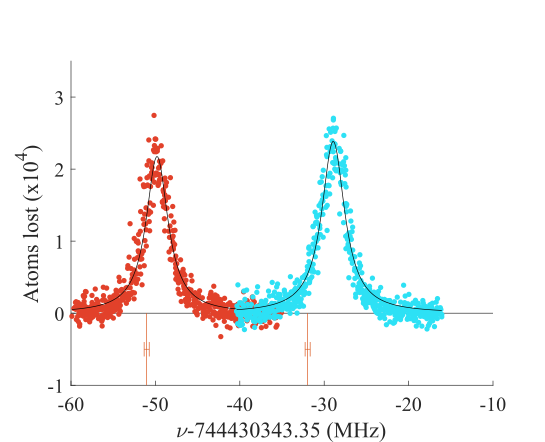
\includegraphics[width=0.65\textwidth]{5^1D_2_plot_combo.png}
%   \caption{Example of observed transition peaks, here a singlet-triplet transition with predicted oscillator strength five orders of magnitude weaker than that of the cooling transition. Left and right peaks are observed absorption peaks with 18G and 11G background fields, respectively.  }
% \end{figure}
% \begin{table}[h]
% \begin{center}
%     \begin{tabular}{|c||c|c|c|p{1cm}}
%     \hline
%         Upper state &  $\nu_{obs}$ (MHz)     & $ \nu_{obs} - \nu_{\textrm{Martin}}\cite{Martin60}$\\
%     \hline\hline
%         $5^3\mathrm{S}_1$    & 727303247(4)        & 13713(201)\\
%         $5^3\mathrm{D}_1$    & 744396515(20)        & 13575(168)\\
%         $5^3\mathrm{D}_2$    & 744396235(20)        & 13855(168)\\
%         $5^3\mathrm{D}_3$    & 744396204(20)        & 13886(168)\\
%         $5^1\mathrm{D}_2$    & 744430345(20)        & N/A\\
%         \hline
%     \end{tabular}
%     \caption{Results of our measurements of transition frequencies between the $2^3\textrm{P}_2$ state to the listed upper states. Uncertainty in observed frequency is dominated by the limiting wavemeter accuracy, and the uncertainty in the difference between new and old values is the combined uncertainty of both measurements.}% Martin method}
% \end{center}
% \end{table}

%% References with bibTeX database:
% \newline

\bibliographystyle{model1-num-names}
\bibliography{bib.bib}

% \newpage

% \section{100 word abstract}
% We report on the first observation of the spin-forbidden 2 3P2- 5 1D2 transition in Helium, and an improvement over historical measurements of the 2 3P2 -- 5 3S1 and 2 3P2 -- 5 3D transitions [3], with an order of magnitude greater precision. We use the novel technique of measuring atom loss from a BEC after disturbing the cooling process with a probe beam. This allows low-background spectroscopy of excited state transitions with controlled magnetic background in ultra-high vacuum. The widths and positions of the observed peak frequencies[1] agree with the theory within experimental error. These measurements constrain  the 5 3D and 5 1D ionization energies of 4He[5] to 150 parts per billion, and the $5^3S$ to 28 parts per billion.

% \section{250 word abstract}

% The advancing precision of modern atomic spectroscopy is beginning to afford optical tests of fundamental physics in helium through, for instance, nuclear charge radii determinations[1]. Among outstanding discrepancies between predicted and observed Helium transition lines and are the 7.5 sigma difference in the N=3 singlet-triplet splitting[2] and the 93 sigma between Drake's predictions[4] and Martin's measurements[3] of the 2 3P2 -- 5 3S1 and 2 3P2 -- 5 3D transitions. The contribution of this work is a resolution of the latter disagreements, with an order of magnitude greater precision, and a contribution to the former in the first measurement of the 1s3p 3P2- 1s5d 1D2 spin-forbidden transition in Helium.  We use a novel technique for direct, low-background laser spectroscopy of excited state transitions in Helium. We apply a probe beam during the production of a trapped Bose-Einstein condensate to disturb an optical cooling stage. Evaporative cooling transduces this stimulus into change in a final atom number, which we measure with our single-atom sensitive detector. This method is, in principle, single-photon sensitive. The experiments were performed in a controlled magnetic field in ultra-high vacuum. The predicted resonance widths and frequencies[1] agree with the observed values within experimental error. These measurements constrain  the 5 3D and 5 1D ionization energies of 4He to 150 parts per billion, and the 5 3S to 28 parts per billion[5].


% Wienczek: Namely, the $2^3P1-2^3P2$ transition to 25kHz determines the fine structure constant to parts-per-billion and the $2^3P-2^3S$ to 1.4kHz, which can determine the nuclear charge radius to below 0.1\%, better than muonic helium Lamb shift. In the former case, the bottleneck is that theory is not sufficiently developed!
% Measured 2L-3D intervals are about 1MHz larger than theory.

% Patkos Measured $2^3S-2^3P$ and $2^3S-2^1S$ transitions give different isotope shifts, which give disparate predictions for the nuclear charge radii in He3 and He4
% The authors find a four-sigma disagreement between their prediction of the difference-of-squares of the nuclear radii and the measured values. There are two results for the $2^3P-2^3S$ transition which differ slightly from each other but significantly from the $2^1S-2^3S$ transition, (1.069(3) and 1.061(3) fm, and 1.027(11) fm, respectively.) 

% We demonstrate a method for spectroscopy from short-lived excited states which uses forced radio evaporation as a transducer between photon scattering events and the population of a Bose-Einstein condensate of Helium in the metastable 23S1 state (He*). Our multichannel plate and delay-line detector stack is sensitive to individual atoms, allowing precise measurements of small differences in atom number. 


\end{document}

